\let\negmedspace\undefined
\let\negthickspace\undefined
\documentclass[journal]{IEEEtran}
\usepackage[a5paper, margin=10mm, onecolumn]{geometry}
%\usepackage{lmodern} % Ensure lmodern is loaded for pdflatex
\usepackage{tfrupee} % Include tfrupee package

\setlength{\headheight}{1cm} % Set the height of the header box
\setlength{\headsep}{0mm}     % Set the distance between the header box and the top of the text

\usepackage{gvv-book}
\usepackage{gvv}
\usepackage{cite}
\usepackage{amsmath,amssymb,amsfonts,amsthm}
\usepackage{algorithmic}
\usepackage{graphicx}
\usepackage{textcomp}
\usepackage{xcolor}
\usepackage{txfonts}
\usepackage{listings}
\usepackage{enumitem}
\usepackage{mathtools}
\usepackage{gensymb}
\usepackage{comment}
\usepackage[breaklinks=true]{hyperref}
\usepackage{tkz-euclide} 
\usepackage{listings}
% \usepackage{gvv}                                        
\def\inputGnumericTable{}                                 
\usepackage[latin1]{inputenc}                                
\usepackage{color}                                            
\usepackage{array}                                            
\usepackage{longtable}                                       
\usepackage{calc}                                             
\usepackage{multirow}                                         
\usepackage{hhline}                                           
\usepackage{ifthen}                                           
\usepackage{lscape}
\begin{document}

\bibliographystyle{IEEEtran}
\vspace{3cm}

\title{10.7.97}
\author{EE25BTECH11049 - Sai Krishna Bakki}
\maketitle
\vspace{-3em}
\textbf{Question:}\\
Let $\vec{P}\brak{a \sec \theta, b \tan \theta}$ and $\vec{Q}\brak{a \sec \phi, b \tan \phi}$, where $\theta + \phi = \pi/2$, be two points on the hyperbola $\frac{x^2}{a^2} - \frac{y^2}{b^2} = 1$. If $(h, k)$ is the point of intersection of the normals at $\vec{P}$ and $\vec{Q}$, then $k$ is equal to?

\solution\\
The equation of the hyperbola is $\frac{x^2}{a^2} - \frac{y^2}{b^2} = 1$. Following the general form for a conic $g(\vec{x}) = \vec{x}^T \vec{V} \vec{x} + 2\vec{u}^T \vec{x} + f = 0$, we can identify the corresponding matrices and vectors for our hyperbola:
\begin{align}
     \vec{V} = \myvec{b^2 & 0 \\ 0 & -a^2}, 
     \vec{u} = \myvec{0 \\ 0}, 
     f = -a^2b^2
\end{align}
The equation of the normal to the conic at a point of contact $\vec{q}$ is given by:
\begin{align}
 \brak{\vec{V}\vec{q} + \vec{u}}^T \vec{R} \brak{\vec{x} - \vec{q}} = 0 
 \end{align}
where $\vec{R}$ is the 90-degree rotation matrix, $\vec{R} = \myvec{0 & -1 \\ 1 & 0}$.\\
The coordinates are $\vec{P} = \myvec{ a \sec \theta \\ b \tan \theta }$.
The equation of the normal at $\vec{P}$ is:
\begin{align}
   \brak{\vec{V}\vec{P} + \vec{u}}^T \vec{R} \brak{\vec{x} - \vec{P}} = 0 \\
    \myvec{ ab^2 \sec \theta & -a^2b \tan \theta } \myvec{ 0 & -1 \\ 1 & 0 } \myvec{ x - a \sec \theta \\ y - b \tan \theta } &= 0 \\
    \myvec{ -a^2b \tan \theta & -ab^2 \sec \theta } \myvec{ x - a \sec \theta \\ y - b \tan \theta } &= 0\\
    \myvec{a\tan\theta&b\sec\theta}\vec{x}&=(a^2 + b^2) \tan \theta \sec \theta
\end{align}
The coordinates are $\vec{Q} = \myvec{ a \sec \phi \\ b \tan \theta }$.
The equation of the normal at $\vec{Q}$ is:
\begin{align}
    \myvec{ -a^2b \tan \phi & -ab^2 \sec \phi } \myvec{ x - a \sec \phi \\ y - b \tan \phi } &= 0\\
    \myvec{a\tan\phi&b\sec\phi}\vec{x}&=(a^2 + b^2) \tan \phi \sec \phi
\end{align}
We are given the condition $\theta + \phi = \pi/2$. We can use this to simplify the second equation.
The intersection point $(h, k)$ must satisfy the normal equations for both P and Q.
\begin{align}
    \myvec{a\tan\theta&b\sec\theta}\myvec{h\\k}&=(a^2 + b^2) \tan \theta \sec \theta\\
    \myvec{a\cot\theta&b\csc\theta}\myvec{h\\k}&=(a^2 + b^2) \cot \theta \csc \theta
    \end{align}
We can solve this linear system for the variables $h$ and $k$ by setting up an augmented matrix.
\begin{align}
\augvec{2}{1}{
a\tan\theta & b\sec\theta & (a^2+b^2)\tan\theta\sec\theta \\
a\cot\theta & b\csc\theta & (a^2+b^2)\cot\theta\csc\theta}
\end{align}
Simplifying to $\sin\theta $ and $\cos\theta$:
\begin{align*}
 \augvec{2}{1}{
a\sin\theta\cos\theta & b\cos\theta & (a^2+b^2)\sin\theta \\
a\sin\theta\cos\theta & b\sin\theta & (a^2+b^2)\cos\theta
}
\end{align*}
\begin{align}
\xrightarrow{R_2\rightarrow R_2-R_1}
 \augvec{2}{1}{
a\sin\theta\cos\theta & b\cos\theta & (a^2+b^2)\sin\theta \\
0 & b(\sin\theta - \cos\theta) & (a^2+b^2)(\cos\theta - \sin\theta)
}
\end{align}
We get the value of k:  
\begin{align}
    k=\frac{(a^2+b^2)(\cos\theta - \sin\theta)}{b(\sin\theta - \cos\theta)}
\end{align}
Assuming $\theta \neq \pi/4$,
\begin{align}
 k  &= -\frac{a^2 + b^2}{b}
\end{align}
\newpage
    \begin{figure}[H]
    \centering
    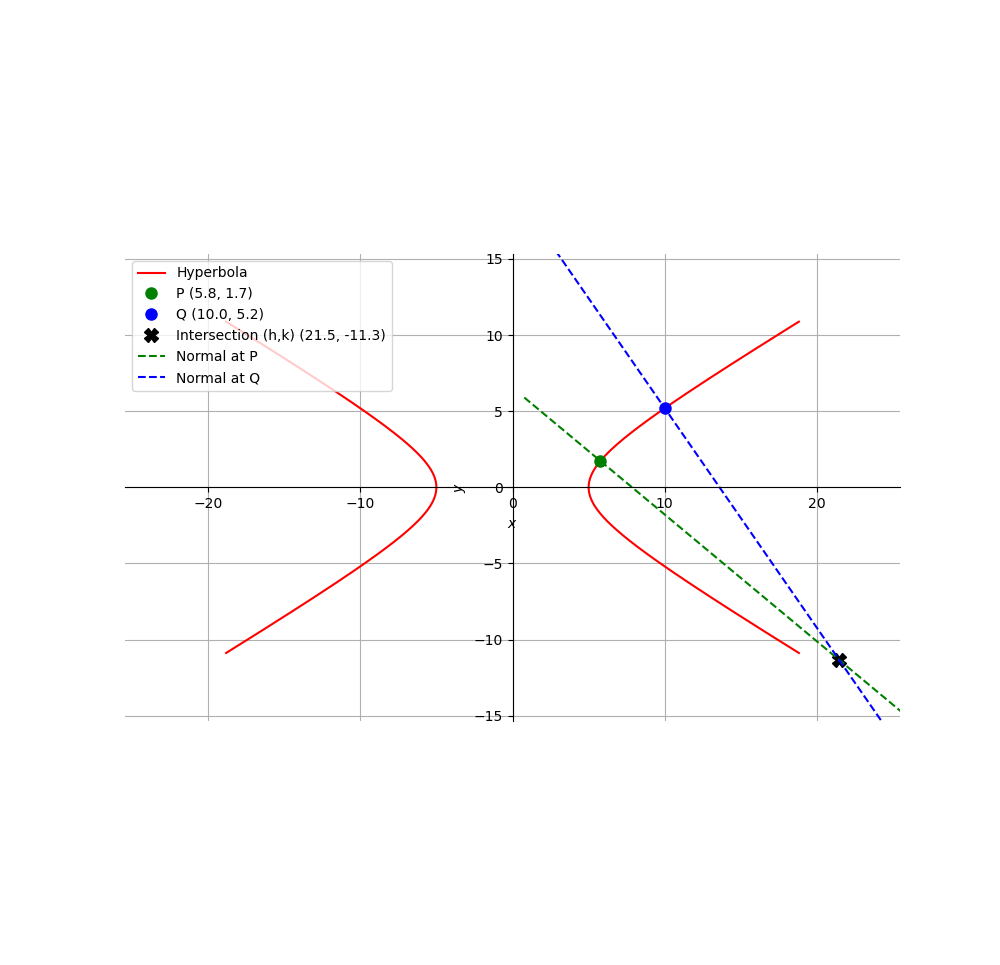
\includegraphics[width=1.1\columnwidth]{figs/Figure_1.png}
    \label{fig:placeholder}
    \caption{}
\end{figure}
\end{document}
